%% template for IEICE Transactions
%% v2.1 [2015/10/31]
\documentclass[paper]{ieice}
%\documentclass[invited]{ieice}
%\documentclass[position]{ieice}
%\documentclass[survey]{ieice}
%\documentclass[invitedsurvey]{ieice}
%\documentclass[review]{ieice}
%\documentclass[tutorial]{ieice}
%\documentclass[letter]{ieice}
%\documentclass[brief]{ieice}
%\usepackage[dvips]{graphicx}
%\usepackage[pdftex]{graphicx,xcolor}
\usepackage[dvipdfmx]{graphicx,xcolor}
\usepackage[fleqn]{amsmath}
\usepackage{newtxtext}
\usepackage[varg]{newtxmath}
\usepackage{bm}
\usepackage{comment}

\setcounter{page}{1}
%\breakauthorline{}% breaks lines after the n-th author

\field{}
%\SpecialIssue{}
%\SpecialSection{}
%\theme{}
\title{Compactness of Finite Union of Regular Patterns and Regular Patterns without Adjacent Variables}
%\title[title for header]{title}
%\titlenote{}
\authorlist{%
\authorentry{Naoto Taketa}{n}{labelA}\MembershipNumber{0000000}
\authorentry{Tomoyuki Uchida}{m}{labelA}\MembershipNumber{9230354}
\authorentry{Takayoshi Shoudai}{m}{labelB}\MembershipNumber{9303359}
\authorentry{Satoshi Matsumoto}{m}{labelC}\MembershipNumber{0307572}
\authorentry{Yusuke Suzuki}{m}{labelA}\MembershipNumber{0120588}
\authorentry{Tetsuhiro Miyahara}{m}{labelA}\MembershipNumber{0401030}
%\authorentry{Takayoshi Shoudai}{m}{labelB}[present affiliate label]\MembershipNumber{}
% \authorentry[e-mail address]{name}{membership}{affiliate label}\MembershipNumber{}
% \authorentry[e-mail address]{name}{membership}{affiliate label}[present affiliate label]\MembershipNumber{}
}
\affiliate[labelA]{Graduate School of Information Sciences, Hiroshima City University}
\affiliate[labelB]{Department of Computer Science and Engineering, Fukuoka
Institute of Technology}
\affiliate[labelC]{Faculty of Science, Tokai University}
%\affiliate[affiliate label]{The author is with the 
%}
%\paffiliate[present affiliate label]{Presently, the author is with the }

\received{2015}{1}{1}
\revised{2015}{1}{1}

%% <local definitions here>
\newtheorem{dfn}{Definition} 
\newtheorem{thm}{Theorem}
\newtheorem{lem}{Lemma}
\newtheorem{col}{Corollary}
\newtheorem{ex}{Example}
\newtheorem{cl}{Claim}
\newenvironment{proof}{\noindent{\bf Proof.}}{\par\medskip}
\renewcommand{\labelenumi}{(\arabic{enumi})}
\newcommand{\proofname}{\textbf{Proof.}}
\newcommand{\qedsymbol}{(Q.E.D)}
%\newcommand{\L}{\mathcal{L}}
\newcommand{\Pat}{\mathcal{P}}
\newcommand{\RPat}{\mathcal{RP}}
\newcommand{\PatL}{\mathcal{P\!\!L}}
\newcommand{\RPatL}{\mathcal{RP\!\!L}}
\newcommand{\Patplus}{\Pat^{+}}
\newcommand{\RPatplus}{\RPat^{+}}
\newcommand{\Patkei}{\Pat^{k}}
\newcommand{\RPatkei}{\RPat^{k}}
\newcommand{\PatLkei}{\PatL^{k}}
\newcommand{\RPatLkei}{\RPatL^{k}}
\newcommand{\NAV}{N\!A\!V}
\newcommand{\NAVR}{\RPat_{N\!A\!V}}
\newcommand{\NAVRPplus}{\RPat^{+}_{N\!A\!V}}
\newcommand{\NAVRPkei}{\RPat^{k}_{N\!A\!V}}

%% </local definitions here>

\begin{document}

\begin{figure*}[t]
  \begin{center}
    %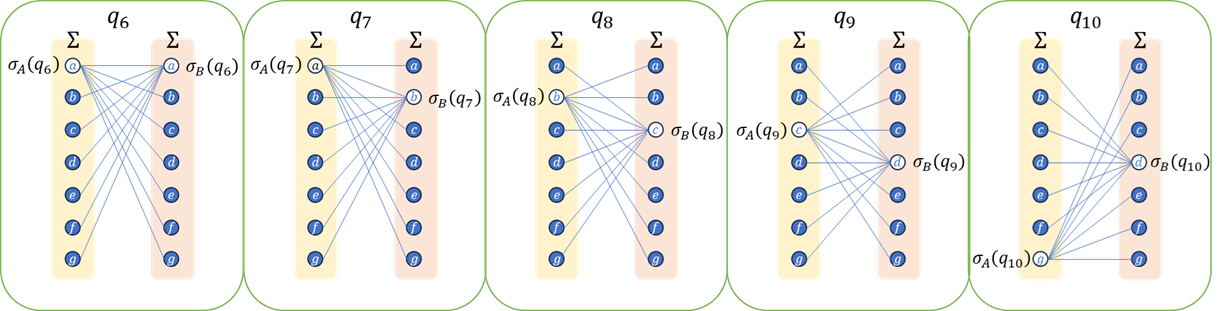
\includegraphics[scale=0.5]{figs/lem8eachreg-suppl.eps}
    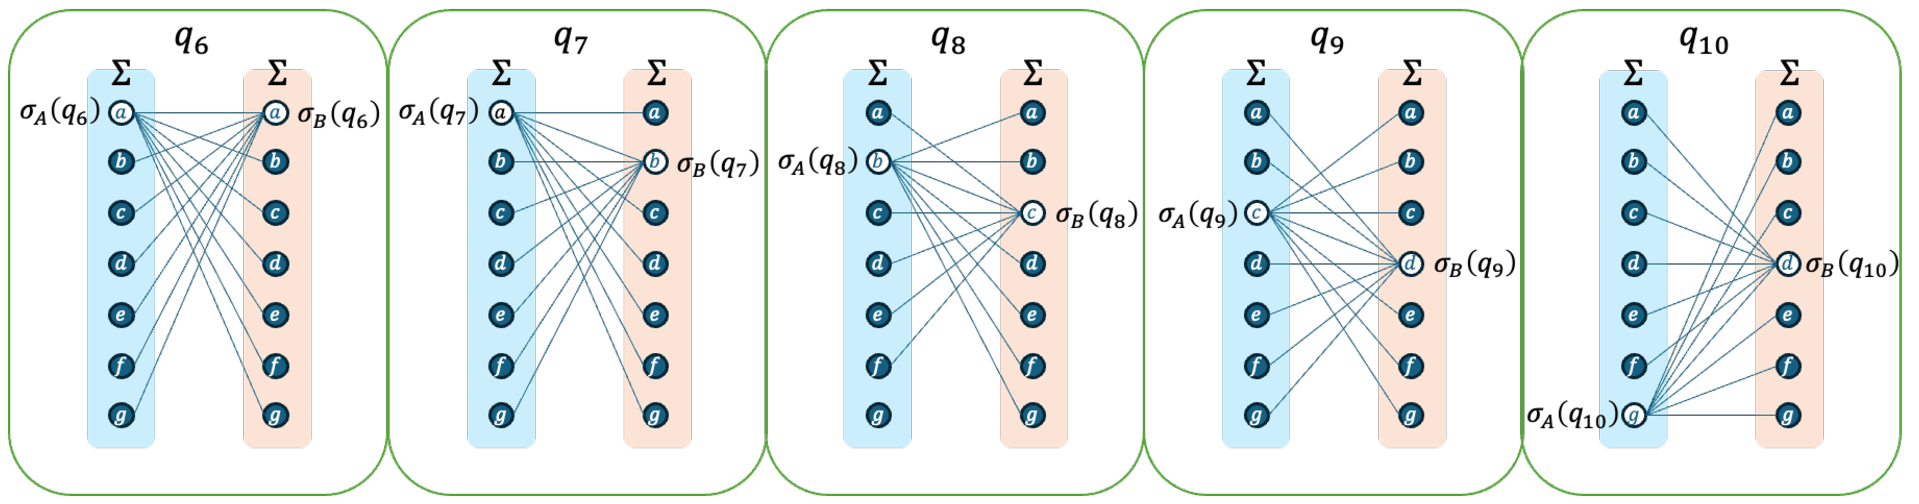
\includegraphics[scale=0.54]{figs/lem8eachreg-suppl.pdf}
    \caption{Let $\Sigma=\{a,b,c,d,e,f,g\}, Q=\{q_6,q_7,q_8,q_9,q_{10}\}$. From these figures, we get $\ell_A=1, \ell_B=1$, $Q^{(\bot,\bot)}=Q^{(\bot,\cdot)}=Q^{(\cdot,\bot)}=\emptyset$, and $Q^{(\cdot,\cdot)}=Q$.}\label{fig:lem8eachreg-suppl}
  \end{center}
\end{figure*}

\begin{figure}[t]
  \begin{center}
    %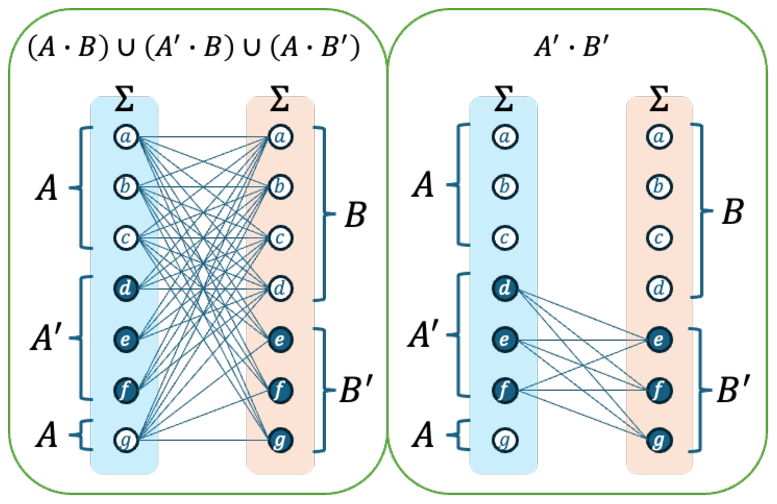
\includegraphics[scale=0.5]{figs/lem8totalreg-suppl.eps}
    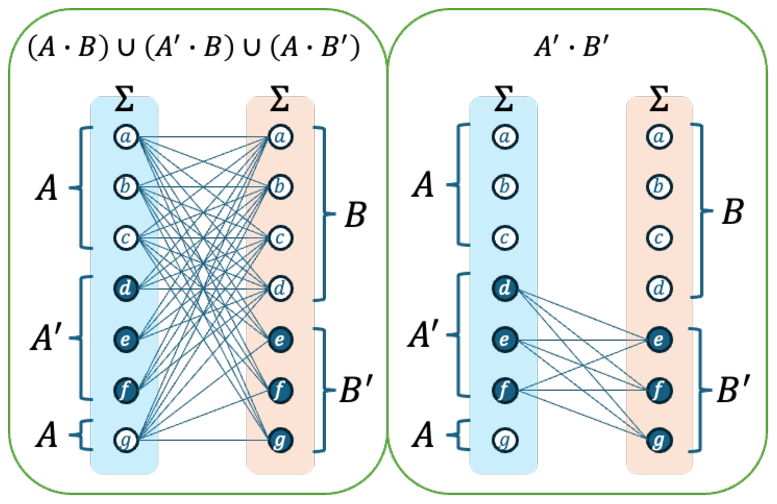
\includegraphics[scale=0.525]{figs/lem8totalreg-suppl.pdf}
    \caption{In the left figure, we aggregate all of the edges appearing in Fig.~\ref{fig:lem8eachreg-suppl}. From Fig.~\ref{fig:lem8eachreg-suppl} and this right figure, we get $Q_{1}^{(\cdot,\cdot)}=\{q_6,q_7,q_8,q_9\}$ and $Q_{2}^{(\cdot,\cdot)}=\{q_{10}\}$. From Proposition~\ref{prop:bothsides}, even if the string $dg \in A'\cdot B'$ satisfies $p \{ x:=gd \} \preceq q_{10}$, it does not imply that $p \{ x:=xy \} \preceq q_{10}$.}\label{fig:lem8totalreg-suppl}
  \end{center}
\end{figure}

\end{document}
